\section{Introduction}
%
A source for deterministic generating entangled photons is a crucial component in the field of quantum information processing. This proposal examines the emission of entangled photon pairs emitted from the biexcition-exciton cascade in a self-assembled quantum dot.  However, the emission of the entangled photons is complicated by the presence of fine structure splitting (FSS)\cite{Winik2017} that leads to the degradation of the degree of entanglement. Many methods were implemented to overcome the problem with varying degrees of success, but the problem persists.\\ 
%
This research proposal aims to take a different approach to the problem by implementing a scheme to restore the degree of entanglement of the photon pairs by fast polarization manipulation \cite{Fognini18,Varo2022}. This scheme can be applied to multiple approaches for generating entangled photons from a QD and enhancing their properties. Furthermore, It can be potentially used as a method for fast photon rerouting in integrated photonics.\\
%
The outline of this research proposal is as follows: The rest of this chapter provides an introduction to quantum dots, their states,
photon correlations, radiative cascades, and a brief description of the problem. Chapter 2 proposes the research that will form the final doctoral thesis. Chapter 3 presents preliminary results and the first steps taken to test our technique.

\subsection{QD 'Artificial Atoms'}
Self-assembled quantum dots (QDs) are localized nano-scale semiconductor structures embedded in a bulk semiconductor, which creates a three-dimensional (3D) potential well in both the valence and conduction bands that can trap charge carriers. Due to their small confinement length relative to the particle's wavelength, the energy levels of the carriers in the QD are quantized with properties similar to atoms which lead them to be described as "Artificial Atoms" \cite{Kastner1993}.\\
%Self-assembled quantum dots (QDs) are localized nano-scale semiconductor structures that create a three-dimensional (3D) potential well in the valence and conduction bands, which trap charge carriers. Due to their small confinement length relative to the particle's wavelength, the energy levels of the QD are quantized with properties similar to atoms which lead them to be described as "Artificial Atoms" \cite{Kastner1993}.\\
%
In recent years, semiconductor QDs were thoroughly investigated as technology-compatible single photon sources, providing a quantum source of "flying qubits" on demand.\cite{Dekel2000,Michler2000,Michler2000_1,Yuan2002}
%Moreover, recently, it has been shown that QDs can emit pair of entangled photons \cite{Akopian2006,Hafenbrak2007} and that an emitted photon can be entangled with the remaining spin in the QD.\cite{Pelk2012,Schaibley2013,Gao2012} These achievements form the required building blocks for quantum information processing. \cite{DiVincenzo1998,Duan2001}
Moreover, it has been recently shown that QDs can emit pair of entangled photons \cite{Akopian2006,Hafenbrak2007} and that an emitted photon can be entangled with the remaining spin in the QD.\cite{Pelk2012,Schaibley2013,Gao2012}
These achievements are required building blocks for quantum information processing.\cite{DiVincenzo1998,Duan2001}
%
\subsection{Entangled photons}
\subsubsection{Definition of Entanglement}
Quantum entanglement is a phenomenon in quantum mechanics where two or more particles can become correlated in such a way that the state of each particle cannot be described independently of the state of the others. 
 In other words, entanglement is the measurement of the separability of a system as described by Peres–Horodecki criterion \cite{Peres1996}.
 %If, on the other hand, the system is prepared in a separable state, then the overall state can be expressed as a product of the states of the individual particles. In this case, the particles are not entangled, and their states can be described independently.
 
\subsubsection{The role of entangled photons in quantum information}
Entanglement is a crucial resource in quantum information processing, enabling key advantages over classical information processing and making possible many of the most exciting and promising applications of quantum technologies.
\textcolor{red}{
\paragraph{Quantum communication}
Quantum communication is about transferring a quantum state from one place to another. Entanglement has a big role in doing that. Entanglement between light and matter performs quantum state transfer and entanglement distribution among distant nodes. Cirac \cite{Circ1997} suggested a protocol in which atoms in a cavity are excited by a laser, mapping the atom state to a photon wave packet that enters a cavity at the receiving node. Quantum repeaters \cite{Briegel1997} correct errors in an entanglement that increase with distance and transmit entangled quantum states over large distances.
\paragraph{Quantum Computation}
Entangled states can be used to perform quantum computation among different nodes in a network. You do not need fixed qubits to do quantum computation. Knill and Milburn \cite{Knill2001} presented a scheme for efficient quantum computation using photons and linear optics. The qubit is one photon with two modes (polarizations H or V), and multiple qubits are basically entangled photon states.
\paragraph{Quantum Key Distribution}
In order to transmit information securely, modern cryptographers require a shared key between the transmitter and the receiver. Arthur Ekert \cite{Ekert1991} presented the E91 protocol, which uses the outcomes of measurements on entangled photon pairs between the sender and receiver to establish a common key. Measuring the Bell inequality for these photon pairs reveals the presence of an eavesdropper.
}
\subsubsection{Fundamental Excitations in QD}
%In semiconductor QDs, at low temperatures, the basic optical excitation, in which an electron is optically excited from the full valence band, thereby leaving there a hole, to the empty conduction band, is called a bright exciton (BE).
%
The basic optical excitation of semiconductor QDs at low temperatures is a bright exciton (BE), where an electron is optically excited from the full valance band to the empty conduction band. The absence of an electron in the valance is called a hole and has an opposite charge and angular momentum of that of the electron. In most self-assembled QDs, the topmost hole's energy state is called a heavy hole with total angular momentum projection of $j^{hh}_z=\pm\frac{3}{2}$, where its orbital angular momentum projection of $\pm 1$ is aligned with its spin. Conversely, the electron in the conduction band has zero orbital angular momentum and total angular momentum projection of $j^e_z=\pm\frac{1}{2}$. Because photons have angular momentum of $1$ and they interact only with the orbital angular momentum of the carriers, the BE is comprised of an electron and heavy-hole pair with anti-parallel angular momentum projection of $j^{BE}_z=\pm 1$.
If the electron and the hole angular momentum projection are aligned, the exciton is called a dark exciton (DE). The total angular momentum projection of the DE is $j^{DE}_z=\pm 2$, and it is optically inactive.
%
In addition, the QD can be occupied by a single charge carrier, either an electron or a hole, or by complexes of charge carriers. For example, a negative Trion comprises two electrons and one hole, while a positive Trion (or negatively charged exciton) comprises one electron and two holes. Another example of an important complex is the biexciton, a complex of two excitons (two electrons and two holes) in the QD.
%In self-assembled QDs, the BE consists of an electron-heavy-hole pair. This optical excitation preserves the excited electron's spin orientation; therefore, the electron and hole have anti-parallel spins. The total angular momentum projection of the BE in the direction of the exciting light is ±1 (like that of the absorbed photon), reflecting the orbital momentum difference between the electron in the valence band to that in the conduction band.
%In most self-assembled QDs, the BE consists of an electron-heavy-hole pair. This optical excitation preserves the excited electron's spin orientation; therefore, the electron and hole have anti-parallel spins. The total angular momentum projection of the BE in the direction of the exciting light is ±1 (like that of the absorbed photon), reflecting the orbital momentum difference between the electron in the valence band to that in the conduction band.
%If the excited conduction electron's spin projection is in addition to the spin projection of the ground valence band electron, the electron and the two holes have parallel spins, with a total angular momentum projection of ±2. This type of excitation is optically forbidden since the light electric field cannot change the electronic spin; therefore, it is called dark exciton (DE). Excitons in the QD can also be generated while the QD contains additional charges, such as a single electron or a single hole. Similarly, many other types of multiple carrier configurations can populate the QD simultaneously. For example, a biexciton is two excitons (two electrons and two holes), and a positively (negatively) charged exciton (trion) is an exciton with the addition of one hole (electron)

\subsubsection{The $\Lambda$ and $\Pi$ systems}
$\Lambda$ system is a three-level physical system in which the two lower eigenstates are coupled to the third eigenstate via an optical transition.
An example Λ system, relevant to this proposal, is presented in Figure \ref{fig:PiSystem}(a), where two BE eigenstates ($\ket{S}= \left( \ket{-1}+\ket{+1} \right)/\sqrt{2}$, and $\ket{A}= \left( \ket{-1}-\ket{+1} \right)/\sqrt{2}$) are coupled to a single biexciton state ($\ket{0}$) with an angular projection of zero.
%$\Lambda$ system is a three-level physical system in which the two eigenstates of a qubit are connected to a third auxiliary level via an optical transition.
%A relevant example to this proposal Λ system is presented in Figure \ref{fig:PiSystem}(a), where the two (degenerate) BE eigenstates are coupled to the ground (non-degenerate) biexciton state.
\begin{figure}[H]
	\centering
	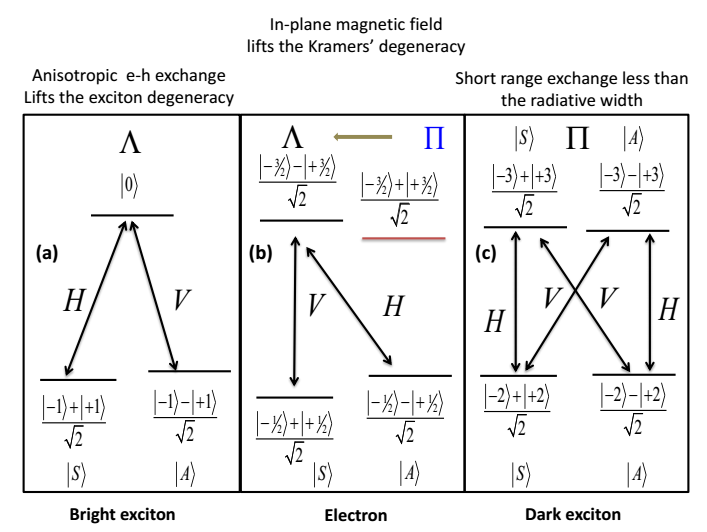
\includegraphics[scale=0.31]{figures/Lambda_System.png}
	\caption{Schematic description of the energy level and selection rules for
optical transition in Λ and Π systems. (a) The BE and the ground biexciton form a $\Lambda$ system. (b) A (degenerate) electron spin forms a $\Pi$ qubit system
with the excited trion states. (c) The (degenerate) DE forms a Π qubit system
with the excited biexciton state. The states are described by their total
angular momentum projections. The arrows symbolize optical transitions, and σ+ (σ-) symbolizes right (left) hand circular polarization.}
	\label{fig:PiSystem}
\end{figure}
A Λ system has physical properties which are very useful for QIP. Notably, since the radiative decay of the auxiliary level to the two ground levels has two paths, the lack of "which-path" information leads to entanglement between the emitted photon polarization and the remaining matter spin qubit. This kind of entanglement between a photon and the exciton was first demonstrated in QDs in 2006 by Akopian et al. \cite{Akopian2006}
%A Λ system has physical properties which are very useful for QIP. Notably, since the radiative decay of the non-degenerate auxiliary level to the qubit has two paths, the lack of "which-path" information leads to entanglement
%between the emitted photon polarization and the remaining matter qubit spin. This kind of entanglement between a photon and matter spin qubit – the exciton was first demonstrated by Akopian et al. \cite{Akopian2006}
%In a $\Pi$ system, the auxiliary level is doubly degenerate, like the qubit is, and two separate optical transitions connect between the qubit to the states of the auxiliary level. An important example is the spin state of a QD confined (Kramers degenerate) electron, and its trion is depicted in Figure \ref{fig:PiSystem}(b).\\
In a $\Pi$ system, the auxiliary level is doubly degenerate, similar to the ground state, while two separate optical transitions couple the ground and the auxiliary levels. An important example of a $\Pi$ system is the spin state of a QD confined electron (Kramers degenerate) and its trion, as depicted in Figure \ref{fig:PiSystem}(b).\\
In Figure \ref{fig:LambdaSystem}, we describe the three systems of Figure \ref{fig:PiSystem} when the degeneracy is removed, either by the EHEI for the exciton (Figure \ref{fig:LambdaSystem}(a) and
(c)), or by an externally applied lateral magnetic field for the electron (Figure \ref{fig:LambdaSystem}).\\
For the Λ system, this degeneracy removal, if it exceeds the radiative decay width, has important consequences. For example, in radiative recombination of the auxiliary state, the decay  which-path information is now expressed in both the polarization of the emitted photon and in the photon energy. Therefore, entanglement between the photon polarization and BE exciton spin requires either spectral filtering \cite{Hafenbrak2007} or temporal filtering \cite{Akopian2006}.\\
Producing entanglement between the emitted photon and the remaining spin in a Π-system is more demanding. Likewise, it is impossible to control the matter-spin using only one optical pulse fully. The way to entangle the polarization of a photon and the spin of the remaining electron is described in Figure \ref{fig:LambdaSystem}. Here, a strong in-plane magnetic field is used to remove the Kramers' degeneracy between the two electron's spin states and the two trion states. If one then uses only one of the trion states as an auxiliary level, a Λ system is formed. Now for achieving photon-spin entanglement, temporal filtering can be used, as recently done by two groups \cite{DeGreve2012} \cite{Schaibley2013}, for obtaining spin - photon-polarization entanglement, or photon polarization filtering \cite{Gao2012} for obtaining spin - photon-energy entanglement.
\begin{figure}[H]
	\centering
	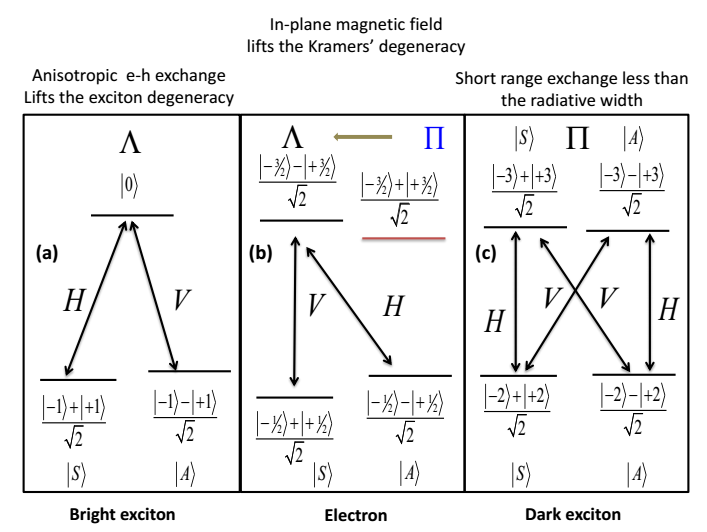
\includegraphics[scale=0.75]{figures/pI_System.png}
	\caption{Schematic description of the energy level and selection rules for
optical transition in non-degenerate $\Lambda$ and $\Pi$ systems. (a) The BE and the ground biexciton auxiliary level as a natural Λ system. (b) The electron spin in the lateral magnetic field as a non-degenerate qubit, forming a $\Lambda$ system (in principle identical to that of the BE) with only one of the trion auxiliary states. (c) The DE and the spin-blockaded biexciton $\Pi$ system, with degeneracy removal by the EHEI. Arrows symbolize resonant optical transitions, and H (V) stands for linear polarization along the major axis of the QD in (a) and (c) and along the direction of the magnetic field in (b).}
	\label{fig:LambdaSystem}
\end{figure}
As shown in Figure \ref{fig:LambdaSystem}c, The DE and its auxiliary biexciton also form a natural Π-system. In this case, however, the degeneracy removal by the EHEI of both the qubit and auxiliary levels is smaller than the radiative width.
\subsubsection{QD as a source of single photon}
Conventional light sources, like lasers, emit radiation that can be successfully described with classical Maxwell equations. On the other hand, quantum communication relies on the availability of light pulses with strong correlations between photons. An example of such an optical source is a single photon emitter, like a semiconductor quantum dot (QD). Semiconductor QDs are nanostructures made of $10^3-10^6$ semiconductor compound unit cells embedded in a higher band-gap semiconductor material. Due to the potential energy difference between the QD and its surrounding material, charge carriers are three-dimensionally confined to the QD, occupying discrete energy levels like in an atom. This fact is very compelling, as the QD is 6 orders of magnitude bigger than an atom, and its charge state can be easily controlled optically or electronically. 
In the year 1999, Gershoni and his group were the first to show that a QD is, in fact, a single photon source \cite{Dekel2000}. A year later, Michler et al.\cite{Michler2000} presented additional supporting evidence for Gershoni's claim. Optical pumping was performed with a mode-locked femtosecond (~250fs) Ti:Sapphire laser operating at 750nm and an 82MHz repetition rate. Hanbury-Brown and Twiss (HBT)-type photon correlation measurements [18] were performed on the QD's bright exciton 950nm emission line. As expected, the measured $g^2(\tau)$  of the pulsed Ti:Sapphire laser (Fig. 2A) exhibited peaks at integer multiples of  $T_{rep} =12.27 nsec$. The measured $g^2(\tau)$ of the exciton emission also showed peaks at integer multiples of $T_{rep}$, indicating the locking of the photon emission to the pulsed excitation. But in contrast to the mode-locked laser, the peak at t=0 is no longer present. That is, the probability of finding a second photon after detecting the first photon at t=0 vanishes.
Numerous applications for using single photon emitters were proposed, though most of them also require consecutive photons to have identical wave packets. Two years after Michler’s publication, Santori et al.cite{Santori2002} showed that a QD is a single photon source, and the photons emitted are indistinguishable. The authors test the indistinguishability of photons emitted by a semiconductor quantum dot in a microcavity through a Hong-Ou-Mandel-type two-photon interference experiment \cite{Fearn:89,DeGreve2012}. When identical single photons enter a 50-50 beam splitter from opposite sides, quantum mechanics requires that both photons must leave in the same direction if their wave packets overlap perfectly. The authors generated single photons by quasi-resonantly exciting a QD twice every 13ns by a pair of equally intense pulses with 2ns separation. The QD emission was collected, and a single polarization was selected. A beam splitter splits the emission into two arms, with one arm 2ns longer than the other. The beam then recombined at a different place on the same beam splitter. Photon counters collected the two outputs of this interferometer, and a photon correlation histogram was generated for the relative delay time $\tau = t_2 - t_1$ of two-photon coincidences. Five peaks appear within the central cluster, corresponding to three types of coincidence events. For the central peak, the first photon follows the long arm, and the second photon follows the short arm such that they collide upon their second pass through the beam splitter. Only in this case can two-photon interference occur, and for perfect two-photon interference, the central peak vanishes.
\subsubsection{The Exciton-Biexciton Cascade (QD as a source of entangled photon pair)}\label{biexciton-exciton-chapter}
The projection of the spin of the electron on the z-axis (growth axis) of the QD can be either 1/2 or -1/2, while for the heavy hole, the spin 
 projection is either 3/2 or -3/2 such that the two spin states of the bright exciton are $\ket{\frac{1}{2},-\frac{2}{3}}$ and $\ket{-\frac{1}
 {2},\frac{2}{3}}$  with a total spin in the z direction  of $\pm1$. While in the case of electron-hole pair with parallel spin, the spin states are $\ket{\frac{1}{2},\frac{2}{3}}$ and $\ket{-\frac{1}{2},-\frac{2}{3}}$ with a total spin of $\pm2$.\\
	In Figure \ref{fig:energy_levels}, we describe two simple configurations we can have in a QD. We start with an empty dot denoted by $\ket{0}$.
	\begin{figure}[H]
		\centering
		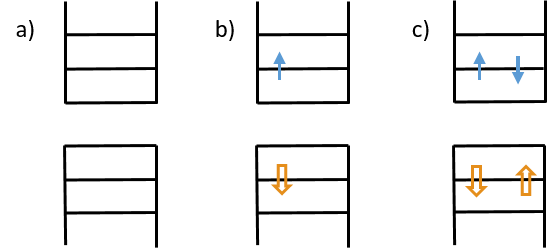
\includegraphics[scale=1]{figures/energy-levels.png}
		\caption{Schematic of the energy levels in the quantum dot for empty quantum dot (a), exciton (b), and a biexciton (c)}
		\label{fig:energy_levels}
	\end{figure}
	while having two electron-hole pairs falling in the dot, a biexciton is formed, and we denote it by $\ket{{XX}_0}$. The total energy of the biexciton differs from twice the energy of the exciton due to the interaction between all the particles.\\
	In an ideal QD, the radiative decay path of the biexciton back to the ground state goes via one path. But due to the anisotropy of the QD, the energy of exciton is split in what is defined as the fine structure splitting (FSS) as seen in Figure \ref{fig:Decay_paths}b. Here we refer to the up (down) spin of the electron as $\ket{\uparrow}$ ($\ket{\downarrow}$ and the up (down) spin of the hole as $\ket{\Uparrow}$ ($\ket{\Downarrow}$ such as the two eigenstates of the exciton are  $\ket{\uparrow\Downarrow}$ and $\ket{\downarrow\Uparrow}$, and the decay from these states result in the emission of photons with co-linear polarization. Here we refer to them as horizontal $\ket{H}$ and vertical $\ket{V}$. We can represent these two rectilinear bases using the Bloch sphere, where the poles in the sphere are $\ket{H}$ and $\ket{V}$ bases.\\
	In addition to the rectilinear polarization states, We can define the diagonal linear and
	the circular polarization bases: 
	\begin{equation}
		\begin{split}
			\ket{L}=(\ket{H}+i\ket{V})/\sqrt{2} \\
			\ket{R}=(\ket{H}-i\ket{V})/\sqrt{2}
		\end{split}
	\end{equation}
	Where $\ket{R}$ and $\ket{L}$ are the left and right circular bases, respectively, and:
	\begin{equation}
		\begin{split}
			\ket{D}=(\ket{H}+\ket{V})/\sqrt{2}\\
			\ket{\bar{D}}=(\ket{H}+\ket{V})/\sqrt{2}
		\end{split}
	\end{equation}
	$\ket{D}$ and $\ket{\bar{D}}$ are the diagonal and anti-diagonal bases respectively
	\begin{figure}[H]
		a)
		\raggedleft
		\def\psiLat{0}
		\def\psiLon{-50}
		\begin{blochsphere}[radius=2.5 cm,tilt=20,rotation=-20,opacity=0]
			\labelLatLon{psi}{\psiLat}{-\psiLon};
			\draw[-latex] (0,0) -- (psi) node[above]{$\large\ket{\psi}$};
			\drawRotationLeft[scale=0.9,style={red}]{0}{0}{0}{15}		
			\drawGreatCircle[style={dashed}]{0}{0}{0}
			\drawBallGrid[style={opacity=0.5}]{30}{30}
			\draw [fill] (0,0) circle (1.5pt);
			\drawGreatCircle[style={dashed}]{0}{0}{0}
			\labelLatLon{up}{90}{0};
			\labelLatLon{down}{-90}{90};
			\node[above] at (up) {{ $\ket{H}$ }};
			\node[below] at (down) {{ $\ket{V}$}};
			\node at (2.8,0) {{$\ket{R}$}};
			\node at (-2.8,0) {{$\ket{L}$}};
			\node at (0,1) {{$\ket{D}$}};
			\node at (0,-1) {{$\ket{\bar{D}}$}};
		\end{blochsphere}
		b)
		\raggedright
		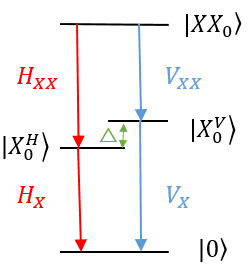
\includegraphics[scale=0.8]{figures/Decay_paths.png}
		\caption{a) A Bloch sphere representation of the spin state. A point on the sphere represents an arbitrarily polarized spin state. b) Decay paths of the biexciton back to the ground state where the red arrows represent the emission of an H-polarized photon and the blue arrows represent the emission of a V-polarized photon.}
		\label{fig:Decay_paths}
	\end{figure}
	When the biexciton spontaneously radiatively decays, it  emits a photon leaving 
	in the QD, an exciton in a coherent superposition of its two eigenstates. The optical
	Selection rules for the biexciton radiative recombination and the lack of information by "which path" the recombination proceeds result in the entanglement between the exciton state and the polarization state of the emitted photon. Their mutual wave function is given by:
	\begin{equation}
		\ket{\psi_{XX^0}} = \frac{1}{\sqrt{2}}(\ket{H_{XX}\otimes\ H_{X}} +\ket{V_{XX} \otimes V_{X}})
	\end{equation}
	Here $\ket{H_{XX}}$($\ket{H_{X}}$) and $\ket{V_{XX}}$($\ket{V_{X}}$) are the two rectilinear polarization states of the biexciton (exciton) photon. However, since the two exciton eigenstates are not degenerate, the relative phase between these eigenstates precesses in time with a period of $T_P = \hslash /\triangle E$, where $\hslash$ is the Planck constant and $\triangle E$ is the exciton FSS \cite{Winik2017}
	This precession is schematically described on the exciton Bloch sphere in Figure. \ref{fig:Decay_paths}(a).
	The precession "stops" when the exciton recombines, and the radiative cascade is completed with the emission of a second photon. The two photons are thus entangled. Their mutual wave function depends on the recombination time and is given by:
	\begin{equation}
		\ket{\psi_{X^0}} = \frac{1}{\sqrt{2}}(\ket{H_{XX}H_{X}} +e^{-i2\pi t/T_P}\ket{V_{XX}V_X})
	\end{equation}
	where $\ket{H_2}$ and $\ket{V_2}$ are the second (exciton) photon polarization states and $t = t_{X_0} - t_{{XX}_0}$ is the time between the emission of the biexciton photon $t_{{XX}_0}$ and that of the exciton $t_{X_0}$. The full therotical treatment for the wavefunction of the two photons from the biexciton-exciton cascade is presented in Appendix \ref{appendix2}.\\
   To evaluate the degree of entanglement between the two photons, we construct the two-photon polarization density matrix from a set of polarized correlations measurements as described in \cite{Kiwat2001}:
   \begin{equation}
   \rho(t) = 
       \begin{pmatrix}
1 & 0 & 0 & e^{-i2\pi \frac{t}{T_P}}\\
0 & 0 & 0 & 0 \\
0 & 0 & 0 & 0 \\
e^{i2\pi \frac{t}{T_P}} & 0 & 0 & 1 
\end{pmatrix}
   \end{equation}
   From the density matrix above, the negativity $\mathcal{N}$ can be calculated, as follows:
   \begin{equation}
		\mathcal{N}[\rho(t)] = \frac{1}{2}\abs{e^{i2\pi \frac{t}{T_P}}} =\frac{1}{2}\abs{e^{i\frac{\triangle E}{\hslash}t}}=\frac{1}{2}
	\end{equation}
 The two photons' polarization states are always maximally entangled from the calculated negativity. However, the state of each pair of photons, which reveals information about the decay path of the radiative cascade, introduces a temporal dependence on the phase in the non-diagonal terms of the density matrix. This temporal dependence has limited resolution $\triangle T$ in an experimental setup.
 \begin{equation}
		\mathcal{N}[\rho(t),\delta T] = \frac{1}{2\triangle T} \abs{\int_t^{t+\triangle T}e^{i2\pi \frac{t^{'}}{T_P}}  dt^{'}}
\end{equation}
where the temporal resolution $\delta T$ is the jitter of the experimental setup. It follows that the measured negativity is independent of the time t:
 \begin{equation}\label{negativity_final}
		\mathcal{N}[\rho(t,\delta T)] = \frac{1}{2} \abs{ sinc \left( \pi \frac{\triangle T}{T_P} \right)}
\end{equation}
As seen from Equation \ref{negativity_final}, the negativity and hence the degree of entanglement vanish for $\triangle T = T_P$, but restore before vanishing at a wider temporal window ($\triangle T \gg T_P$).\\
In Figure \ref{Entanglement1}, The  negativity from experimental data is plotted in blue and fitted calculations in black as a function of the time difference between the emission of the biexciton and exciton photons, where the time zero represents the emission time of the exciton, with a temporal window width of $\Delta T = 24ps$ \cite{Winik2017}. 
 \begin{figure}
	\centering
	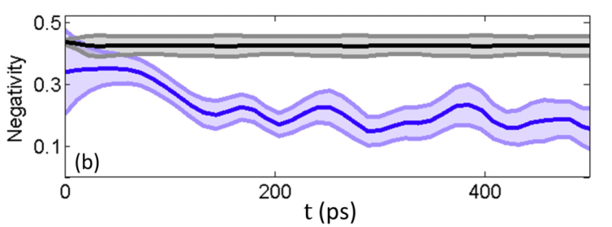
\includegraphics[scale=0.85]{figures/Entanglement_Integration1.png}
	\caption{The negativity of the two-photon polarization density matrix as a function of the time difference between the exciton and biexciton detection times for temporal window width of T = 24ps. The blue line presents the negativity deduced directly from the measured raw data. The black line presents the negativity deduced from the fitted calculations considering the system response. graph taken from \cite{Winik2017}}.
  \label{Entanglement1}
\end{figure}
In Figure \ref{Entanglement2}, the two photons' negativity is a function of the temporal windows $\Delta T$. The blue line represents the negativity calculated from measured data, the black line represents the negativity from the fitted calculations, and the green line represents the theoretical dependence. 
 \begin{figure}[H]
	\centering
	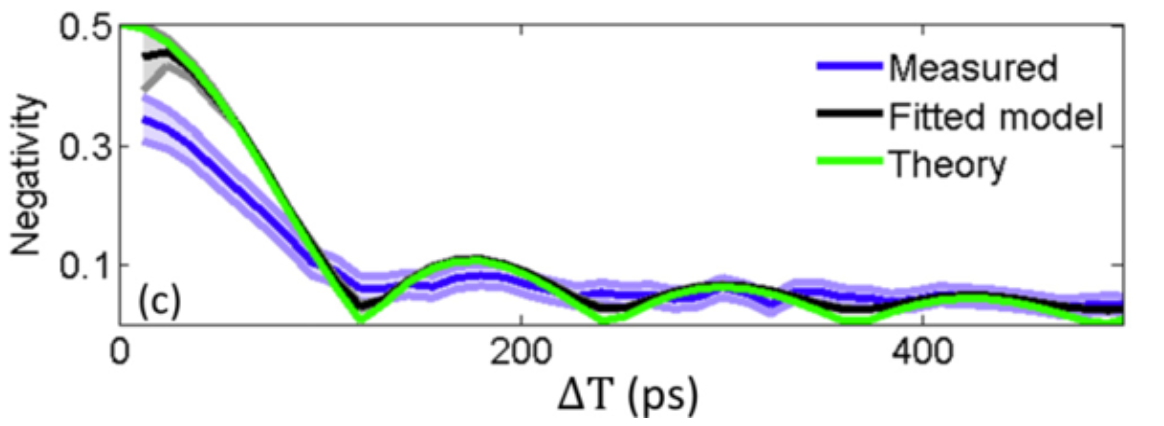
\includegraphics[scale=0.45]{figures/Entanglement_Integration2.png}
	\caption{The negativity of the two photons' polarization density matrix as a function of the temporal window width, T. The blue line presents the negativity deduced directly from the measured raw data. The black line presents the negativity deduced from the fitted calculations, considering the response function solid green solid line represents the theoretical dependence calculated. Shaded areas with corresponding colors represent experimental uncertainties of one standard deviation. graph taken from \cite{Winik2017}}.
   \label{Entanglement2}
\end{figure} 
The measured degree of entanglement between the polarization states of the two photons is affected by the temporal resolution by which the time difference between the two-photon emissions is determined. By constructing a device that can rotate the polarization of the emitted exciton photon, we can restore the entanglement between the two photons and transform any quantum dot into an on-demand source of maximally entangled photons.
\subsubsection{QD Spin as a Generator for a String of Entangled Photons}
Another technique to produce entangled photons from a QD is based on Lindner and Rudolph's proposal for generating one-dimensional photonic cluster states \cite{Linder2009}. This proposal is based on the spin of a single charge carrier confined precessing using an external magnetic field and driven by sequential laser pulses. After each pulse, a  single deterministic photon is emitted, and its polarization is entangled with the spin of the charge carrier. This process can be theoretically repeated to generate an infinite string of entangled photons.\\
Recently, Cogan et al.\cite{Cogan2023} demonstrated generating a cluster state using this protocol by entangling the photons with the spin of a single heavy hole in a QD, with a characteristic entanglement length of ten photons and a photon indistinguishability close to $80 \%$. This technique can be further enhanced by obtaining a better collection efficiency and reducing the emission lifetime.   
\subsection{Optimized Platforms for the Emission from a QD}
Quantum optic technologies require a bright source of entangled photons. The emission from a QD is enhanced by placing it in photonic structures such as a cavity. This leads to a higher Purcell factor and increases signal extraction efficiency. An emerging approach is using circular Bragg grating (CBG)\cite{Davanço2011}, which can obtain an extraction efficiency above 90\% and a Purcell factor higher than 20\cite{Jian-Wei2019}.\\
Another promising approach is a tunable open Fabry–Perot microcavities\cite{Sumetsky2019}. This unique approach allows in situ tunability by moving a mirror to the required optical resonance frequency with high precision. In addition, this type of microcavity offers a high-quality factor per volume and, therefore, a strong light-matter interaction \cite{Flagan:22}.